% !TEX root = ../main.tex
\section{Shortcomings of Text-Based Authentication} \label{sec:shortcomings}

  User authentication is a central part of security systems. Despite the extensive number of options for authentication, text-based passwords remain the most common authentication scheme. Text-based authentication is the authentication scheme widely adopted because it is easy and inexpensive to implement, and users are familiar with the scheme. Text-based authentication also avoids the privacy issues raised by the use of biometric authentication, as well as preventing the need for a physical security device used in token-based authentication schemes. However, text-based authentication suffers from both security and usability disadvantages. As users need to remember an increasing number of passwords, users adopt bad password habits. The term {\it habit} is often a bad thing when talking about security. A habit is often hard to change and is often predictable because it tends to occur in similar situations repeatedly.

  Password reuse is one of the known password habits among users, caused by human limitations for being able to remember text-based passwords.Another habit introduced as a cause of dealing with the problem of remembering passwords is to create short and meaningful passwords that are easier to remember. However, a consequence of creating short passwords is a vulnerability for brute-force attacks, introducing a security risk. Furthermore, having an expanding number of accounts requires users to manage a set of different passwords across multiple devices. The problem is not just to remember all the required passwords, but also to remember which passwords belong to which account or device. The increased number of accounts and devices is an another cause for users to reuse passwords across multiple accounts and devices.

  One of the first large-scale studies on web password habits was conducted in 2007 by Microsoft Research \cite{habits1}. They analyzed text-based passwords used by 544.960 Internet users over a period of 3 months. In order to collect the passwords, Microsoft used a Windows Live Toolbar observing activities like login frequency. They were also able to observe how many unique passwords each user had and how the passwords were used across separate URLs. Microsoft observed that a typical user has an average of 7 distinct passwords. Out of the seven unique passwords, five of them were re-used on different web pages. An estimate of the average number of accounts per user was estimated to 25 accounts per user.

  Password schemes have what is called a {\it theoretical password space} that is the number of possible combinations of passwords that a user can make. Research has reported that when creating passwords, users to not utilize the entire password space, but uses only a subset of the conceivable password combinations. The password space in use can be seen as the {\it practical password space}, making the practical password space less than the theoretical password space (Figure \ref{fig:memorable}). The selected passwords show that the security of a password scheme relates to its practical password space rather than its theoretical password space.

    \begin{figure}[H]
      \centering
      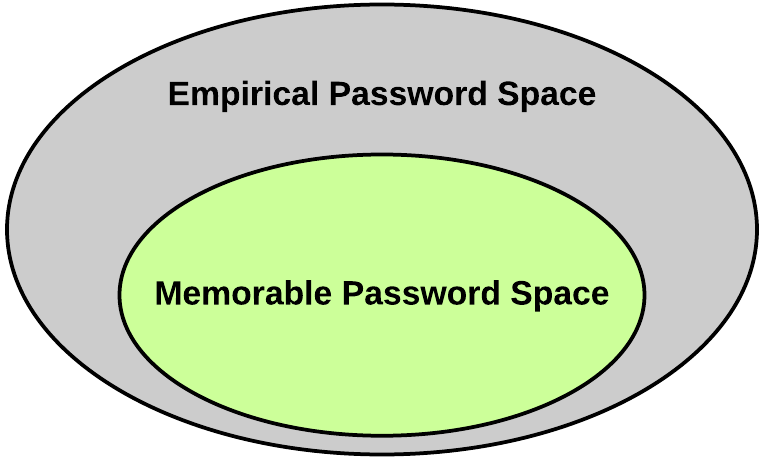
\includegraphics[scale=0.55]{pics/review/EmpiricalVsPractical.png}
      \caption{Theoretical password space vs. Password space in practice}
      \label{fig:memorable}
    \end{figure}

  In a case study of 14.000 Unix passwords, a research group found that 25\% of the passwords were a group of words forming a dictionary of $3\times10^{6}$ words \cite{UnixPasswords}. This dictionary shows that an attacker can have a relatively high success rate for an attack, despite the fact that there are roughly $2\times10^{14}$ 8-character passwords consisting of digits, and upper and lower case letters. As a result of people choosing weak passwords that are easier to remember, a significant number of user-chosen passwords falls into a small dictionary, e.g. the password space in practice \cite{Tao}. A well-designed dictionary is considered to be a tiny subset of the full password space, e.g. the theoretical password space, which further may be prioritized according to the likelihood for a password to be chosen. It is, therefore, commonly stated that the security of a password scheme is related to the size of its password space in practice, rather than its theoretical password space. The high success rate of dictionary attacks against text-based passwords is considered to be a significant cause of the recall capabilities of humans and how they choose their passwords.

  As a result of the shortcomings of text-based authentication, graphical authentication is getting increased attention as an alternative to text-based authentication. Graphical passwords are attempting to help the users to be able to create secure passwords that are also easy to remember. Instead of consisting of text and numbers, graphical passwords make use of images and visual objects in the authentication process. When comparing the use of text against the use of visual objects, the human brain is more capable of remembering images than text \cite{DeAngeli}. As a consequence of humans being more capable of recognizing images, users will be more capable of creating more complicated passwords that are harder to guess.

  The next section will look further into the history of graphical passwords; when did it all start and what does the situation look like today?
  